% !TeX root = ../main.tex
\chapter{Detailed Class Diagrams}
\label{appendix:class-diagrams}

The Content Authoring class diagram is presented in
Chapter~\ref{chap:phan-tich-thiet-ke} because it carries the Lesson
aggregate -- the unit of LTI Deep Linking and the most architecturally
load-bearing entity. The Curriculum bounded context is provided here
for completeness.

\section{Curriculum Bounded Context}
\label{appendix:class-curriculum}

The curriculum context models the CDIO/Bloom course structure.
\texttt{LearningOutcome} is versioned by \texttt{academic\_year} so
that the Knowledge Graph evolves as the curriculum changes year by
year -- the novelty contribution of this project. \texttt{Chunk} from
the Content Authoring context is referenced through the
\texttt{ChunkLOMapping} join table to keep the two contexts decoupled.

\begin{figure}[H]
    \centering
    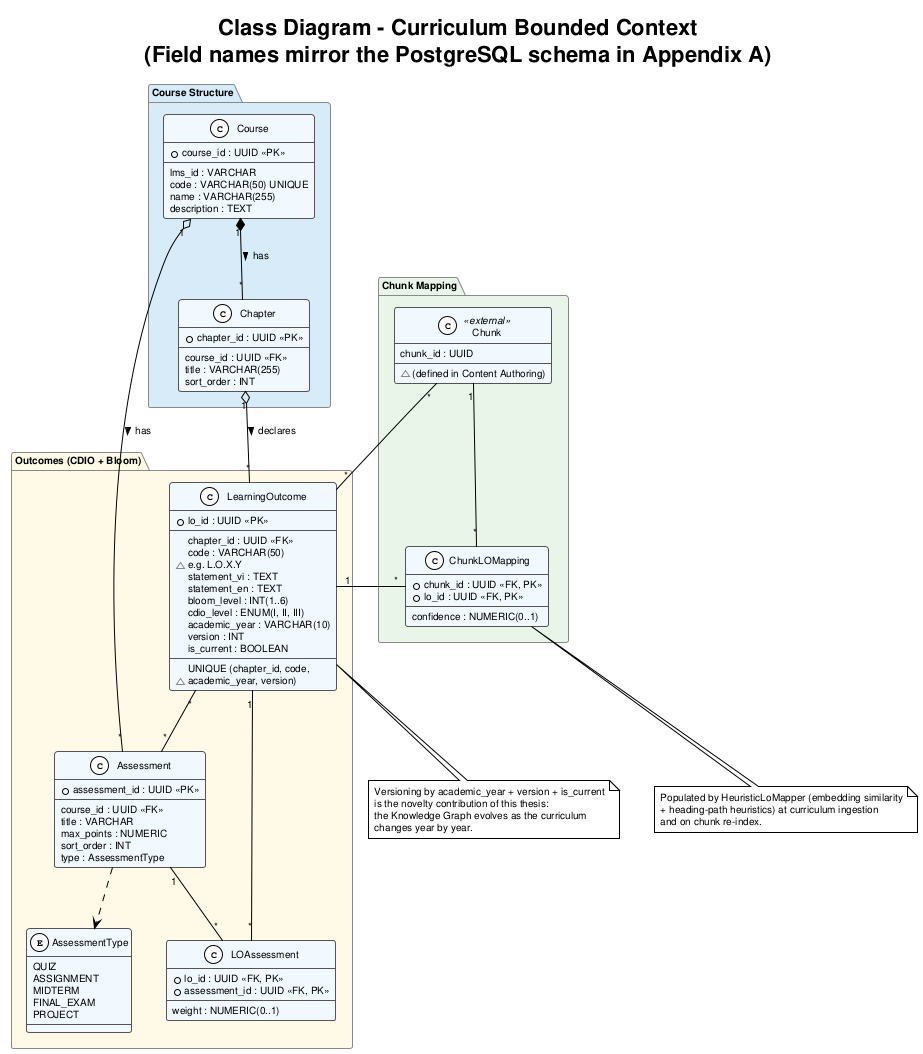
\includegraphics[width=\textwidth,height=0.88\textheight,keepaspectratio]{diagrams/class_diagram_curriculum.png}
    \caption{Class diagram of the Curriculum bounded context.}
    \label{fig:class-curriculum}
\end{figure}
